\subsubsection{x86: 3 arguments entier}

\myparagraph{MSVC}

En le compilant avec MSVC 2010 Express nous obtenons:

\begin{lstlisting}[style=customasmx86]
$SG3830	DB	'a=%d; b=%d; c=%d', 00H

...

	push	3
	push	2
	push	1
	push	OFFSET $SG3830
	call	_printf
	add	esp, 16					; 00000010H
\end{lstlisting}

Presque la même chose, mais maintenant nous voyons que les arguments de \printf sont
poussés sur la pile en ordre inverse. Le premier argument est poussé en dernier.

À propos, dans un environnement 32-bit les variables de type \Tint ont une taille
de 32-bit. ce qui fait 4 octets.

Donc, nous avons 4 arguments ici. $4*4 = 16$~---ils occupent exactement 16 octets
dans la pile: un pointeur 32-bit sur une chaîne et 3 nombres de type \Tint.

\myindex{x86!\Instructions!ADD}
\myindex{x86!\Registers!ESP}
\myindex{cdecl}
Lorsque le \glslink{stack pointer}{pointeur de pile} (registre \ESP) est re-modifié
par l'instruction \INS{ADD ESP, X} après un appel de fonction, souvent, le nombre
d'arguments de la fonction peut-être déduit en divisant simplement X par 4.

Bien sûr, cela est spécifique à la convention d'appel \emph{cdecl}, et seulement
pour un environnement 32-bit.

Voir aussi la section sur les conventions d'appel ~(\myref{sec:callingconventions}).

Dans certains cas, plusieurs fonctions se terminent les une après les autres, le
compilateur peut concaténer plusieurs instructions \q{ADD ESP, X} en une seule,
après le dernier appel:

\begin{lstlisting}[style=customasmx86]
push a1
push a2
call ...
...
push a1
call ...
...
push a1
push a2
push a3
call ...
add esp, 24
\end{lstlisting}

Voici un exemple réel:

\lstinputlisting[caption=x86,style=customasmx86]{patterns/03_printf/x86/add_example_FR.lst}

\clearpage
\myparagraph{MSVC et \olly}
\myindex{\olly}

Maintenant, essayons de charger cet exemple dans \olly.
C'est l'un des débuggers en espace utilisateur win32 les plus populaire.
Nous pouvons compiler notre exemple avec l'option \GTT{/MD} de MSVC 2012, qui signifie
lier avec \GTT{MSVCR*.DLL}, ainsi nous verrons clairement les fonctions importées
dans le debugger.

Ensuite chargeons l'exécutable dans \olly.
Le tout premier point d'arrêt est dans \GTT{ntdll.dll}, appuyez
sur F9 (run).
Le second point d'arrêt est dans le code \ac{CRT}.
Nous devons maintenant trouver la fonction \main.

Trouvez ce code en vous déplaçant au tout début du code (MSVC alloue la fonction
\main au tout début de la section de code):
\begin{figure}[H]
\centering
\myincludegraphics{patterns/03_printf/x86/olly3_1.png}
\caption{\olly: le tout début de la fonction \main}
\label{fig:printf3_olly_1}
\end{figure}

Clickez sur l'instruction \INS{PUSH EBP}, pressez F2 (mettre un point d'arrêt)
et pressez F9 (lancer le programme).
Nous devons effectuer ces actions pour éviter le code \ac{CRT}, car il ne nous intéresse
pas pour le moment.

\clearpage
Presser F8 (\stepover) 6 fois, i.e. sauter 6 instructions:

\begin{figure}[H]
\centering
\myincludegraphics{patterns/03_printf/x86/olly3_2.png}
\caption{\olly: avant l'exécution de \printf}
\label{fig:printf3_olly_2}
\end{figure}

Maintenant le \ac{PC} pointe vers l'instruction \INS{CALL printf}.
\olly, comme d'autres debuggers, souligne la valeur des registres qui ont changé.
Donc, chaque fois que vous appuyez sur F8, \EIP change et sa valeur est affichée en rouge.
\ESP change aussi, car les valeurs des arguments sont poussées sur la pile.\\
\\
Où sont les valeurs dans la pile?
Regardez en bas à droite de la fenêtre du debugger:

\begin{figure}[H]
\centering
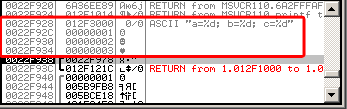
\includegraphics[width=0.5\textwidth]{patterns/03_printf/x86/olly3_stack.png}

\caption{\olly: pile après que les valeurs des arguments aient été poussées (Le
rectangle rouge a été ajouté par l'auteur dans un éditeur graphique)}
\end{figure}

Nous pouvons voir 3 colonnes ici: adresse dans la pile, valeur dans la pile et quelques
commentaires additionnels d'\olly.
\olly peut détecter les pointeurs sur des chaînes ASCII dans la pile, donc il
rapporte la chaîne de \printf{} ici.

Il est possible de faire un clic-droit sur la chaîne de format, cliquer sur \q{Follow in dump},
et la chaîne de format va apparaître dans la fenêtre en bas à gauche du debugger. qui affiche
toujours des parties de la mémoire.
Ces valeurs en mémoire peuvent être modifiées.
Il est possible de changer la chaîne de format, auquel cas le résultat de notre
exemple sera différent.
Cela n'est pas très utile dans le cas présent, mais ce peut-être un bon exercice
pour commencer à comprendre comment tout fonctionne ici.

\clearpage
Appuyer sur F8 (\stepover).

Nous voyons la sortie suivante dans la console:

\lstinputlisting{patterns/03_printf/x86/console.txt}

Regardons comment les registres et la pile ont changés:

\begin{figure}[H]
\centering
\myincludegraphics{patterns/03_printf/x86/olly3_3.png}
\caption{\olly après l'exécution de \printf{}}
\label{fig:printf3_olly_3}
\end{figure}

Le registre \EAX contient maintenant \GTT{0xD} (13).
C'est correct, puisque \printf renvoie le nombre de caractères écrits.
La valeur de \EIP a changé: en effet, il contient maintenant l'adresse de l'instruction
venant après
\INS{CALL printf}.
Les valeurs de \ECX et \EDX ont également changé.
Apparemment, le mécanisme interne de la fonction \printf les a utilisés pour dans
ses propres besoins.

Un fait très important est que ni la valeur de \ESP, ni l'état de la pile n'ont
été changés!
Nous voyons clairement que la chaîne de format et les trois valeurs correspondantes
sont toujours là.
C'est en effet le comportement de la convention d'appel \emph{cdecl}: \glslink{callee}{l'appelée}
ne doit pas remettre \ESP à sa valeur précédente.
\glslink{caller}{L'appelant} est responsable de le faire.

\clearpage
Appuyer sur F8 à nouveau pour exécuter l'instruction \INS{ADD ESP, 10}:

\begin{figure}[H]
\centering
\myincludegraphics{patterns/03_printf/x86/olly3_4.png}
\caption{\olly: après l'exécution de l'instruction \INS{ADD ESP, 10}}
\label{fig:printf3_olly_4}
\end{figure}

\ESP a changé, mais les valeurs sont toujours dans la pile!
Oui, bien sûr; il n'y a pas besoin de mettre ces valeurs à zéro ou quelque chose
comme ça.
Tout ce qui se trouve au dessus du pointeur de pile (\ac{SP}) est du \emph{bruit}
ou des \emph{déchets} et n'a pas du tout de signification.
Ça prendrait beaucoup de temps de mettre à zéro les entrées inutilisées de la
pile, et personne n'a vraiment besoin de le faire.

\myparagraph{GCC}

Maintenant, compilons la même programme sous Linux en utilisant GCC 4.4.1 et regardons
ce que nous obtenons dans \IDA:

\lstinputlisting[style=customasmx86]{patterns/03_printf/x86/x86_1.asm}

Il est visible que la différence entre le code MSVC et celui de GCC est seulement
dans la manière dont les arguments sont stockés sur la pile.
Ici GCC manipule directement la pile sans utiliser \PUSH/\POP.

\myparagraph{GCC et GDB}
\myindex{GDB}

Essayons cet exemple dans \ac{GDB} sous Linux.

L'option \GTT{-g} indique au compilateur d'inclure les informations de debug dans
le fichier exécutable.

\begin{lstlisting}
$ gcc 1.c -g -o 1
\end{lstlisting}

\begin{lstlisting}
$ gdb 1
GNU gdb (GDB) 7.6.1-ubuntu
...
Reading symbols from /home/dennis/polygon/1...done.
\end{lstlisting}

\begin{lstlisting}[caption=let's set breakpoint on \printf]
(gdb) b printf
Breakpoint 1 at 0x80482f0
\end{lstlisting}

Lançons le programme.
Nous n'avons pas la code source de la fonction \printf ici, donc \ac{GDB} ne peut
pas le montrer, mais pourrait.

\begin{lstlisting}
(gdb) run
Starting program: /home/dennis/polygon/1

Breakpoint 1, __printf (format=0x80484f0 "a=%d; b=%d; c=%d") at printf.c:29
29	printf.c: No such file or directory.
\end{lstlisting}

Afficher 10 éléments de la pile. La colonne la plus à gauche contient les adresses
de la pile.

\begin{lstlisting}
(gdb) x/10w $esp
0xbffff11c:	0x0804844a	0x080484f0	0x00000001	0x00000002
0xbffff12c:	0x00000003	0x08048460	0x00000000	0x00000000
0xbffff13c:	0xb7e29905	0x00000001
\end{lstlisting}

Le tout premier élément est la \ac{RA} (\GTT{0x0804844a}).
Nous pouvons le vérifier en désassemblant la mémoire à cette adresse:

\begin{lstlisting}[label=NOP_as_XCHG_example,style=customasmx86]
(gdb) x/5i 0x0804844a
   0x804844a <main+45>:	mov    $0x0,%eax
   0x804844f <main+50>:	leave  
   0x8048450 <main+51>:	ret    
   0x8048451:	xchg   %ax,%ax
   0x8048453:	xchg   %ax,%ax
\end{lstlisting}

Les deux instructions \INS{XCHG} sont des instructions sans effet, analogues à \ac{NOP}s.

Le second élément (\GTT{0x080484f0}) est l'adresse de la chaîne de format:

\begin{lstlisting}
(gdb) x/s 0x080484f0
0x80484f0:	"a=%d; b=%d; c=%d"
\end{lstlisting}

Les 3 éléments suivants (1, 2, 3) sont les arguments de \printf.
Le reste des éléments sont juste des \q{restes} sur la pile, mais peuvent aussi
être des valeurs d'autres fonctions, leurs variables locales, etc.
Nous pouvons les ignorer pour le moment.

Lancer la commande \q{finish}.
Cette commande ordonne à GDB d'\q{exécuter toutes les instructions jusqu'à la
fin de la fonction}.
Dans ce cas: exécuter jusqu'à la fin de \printf.

\begin{lstlisting}
(gdb) finish
Run till exit from #0  __printf (format=0x80484f0 "a=%d; b=%d; c=%d") at printf.c:29
main () at 1.c:6
6		return 0;
Value returned is $2 = 13
\end{lstlisting}

\ac{GDB} montre ce que \printf a renvoyé dans \EAX (13).
C'est le nombre de caractères écrits, exactement comme dans l'exemple avec \olly.

Nous voyons également \q{return 0;} et l'information que cette expression se trouve
à la ligne 6 du fichier \GTT{1.c}.
En effet, le fichier \GTT{1.c} se trouve dans le répertoire courant, et \ac{GDB}
y a trouvé la chaîne.
Comment est-ce que \ac{GDB} sait quelle ligne est exécutée à un instant donné?
Cela est du au fait que lorsque le compilateur génère les informations de debug,
il sauve également une table contenant la relation entre le numéro des lignes du
code source et les adresses des instructions.
GDB est un debugger niveau source, après tout.

Examinons les registres.
13 in \EAX:

\begin{lstlisting}
(gdb) info registers
eax            0xd	13
ecx            0x0	0
edx            0x0	0
ebx            0xb7fc0000	-1208221696
esp            0xbffff120	0xbffff120
ebp            0xbffff138	0xbffff138
esi            0x0	0
edi            0x0	0
eip            0x804844a	0x804844a <main+45>
...
\end{lstlisting}

Désassemblons les instructions courantes.
La flèche pointe sur la prochaine instruction qui sera exécutée.

\begin{lstlisting}[style=customasmx86]
(gdb) disas
Dump of assembler code for function main:
   0x0804841d <+0>:	push   %ebp
   0x0804841e <+1>:	mov    %esp,%ebp
   0x08048420 <+3>:	and    $0xfffffff0,%esp
   0x08048423 <+6>:	sub    $0x10,%esp
   0x08048426 <+9>:	movl   $0x3,0xc(%esp)
   0x0804842e <+17>:	movl   $0x2,0x8(%esp)
   0x08048436 <+25>:	movl   $0x1,0x4(%esp)
   0x0804843e <+33>:	movl   $0x80484f0,(%esp)
   0x08048445 <+40>:	call   0x80482f0 <printf@plt>
=> 0x0804844a <+45>:	mov    $0x0,%eax
   0x0804844f <+50>:	leave  
   0x08048450 <+51>:	ret    
End of assembler dump.
\end{lstlisting}

\ac{GDB} utilise la syntaxe AT\&T par défaut.
Mais il est possible de choisir la syntaxe Intel:

\begin{lstlisting}[style=customasmx86]
(gdb) set disassembly-flavor intel
(gdb) disas
Dump of assembler code for function main:
   0x0804841d <+0>:	push   ebp
   0x0804841e <+1>:	mov    ebp,esp
   0x08048420 <+3>:	and    esp,0xfffffff0
   0x08048423 <+6>:	sub    esp,0x10
   0x08048426 <+9>:	mov    DWORD PTR [esp+0xc],0x3
   0x0804842e <+17>:	mov    DWORD PTR [esp+0x8],0x2
   0x08048436 <+25>:	mov    DWORD PTR [esp+0x4],0x1
   0x0804843e <+33>:	mov    DWORD PTR [esp],0x80484f0
   0x08048445 <+40>:	call   0x80482f0 <printf@plt>
=> 0x0804844a <+45>:	mov    eax,0x0
   0x0804844f <+50>:	leave  
   0x08048450 <+51>:	ret    
End of assembler dump.
\end{lstlisting}

Exécuter la ligne suivante de code \CCpp{}.
\ac{GDB} montre une parenthèse fermante, signifiant la fin du bloc.

\begin{lstlisting}
(gdb) step
7	};
\end{lstlisting}

Examinons les registres après l'exécution de l'instruction \INS{MOV EAX, 0}.
En effet, \EAX est à zéro à ce stade.

\begin{lstlisting}
(gdb) info registers
eax            0x0	0
ecx            0x0	0
edx            0x0	0
ebx            0xb7fc0000	-1208221696
esp            0xbffff120	0xbffff120
ebp            0xbffff138	0xbffff138
esi            0x0	0
edi            0x0	0
eip            0x804844f	0x804844f <main+50>
...
\end{lstlisting}

